\cleardoublepage
\chapter{Software}
% To do: 
% Color Scheme
% Red - Not started
% Yellow - In progress
% Blue - Done, under approval
% Green - Done and approved
\todo[inline,color=red!40]{*Chapter Introduction}
\todo[inline,color=red!40]{*1 - Microphone}
\todo[inline,color=red!40]{ a) WOMic}
\todo[inline,color=red!40]{ b) MatLab}
\todo[inline,color=red!40]{*2 - Accelerometer and Piezoelectric}
\todo[inline,color=red!40]{ a) Microcontroller}
\todo[inline,color=red!40]{ b) MatLab}
\todo[inline,color=red!40]{ c) FFT implementation}
%% Writing %%%%%%%%%%%%%%%%%%%%%%%%%%%%%%%%%%%%%%%%%%%%%%%%%%%%%%%%%%%%
\section{Microphone}
\subsection{WOMic}
\subsection{MatLab}
\section{Accelerometer and Piezoelectric}
\subsection{Microcontroller}
\subsection{MatLab}
\subsection{FFT implementation}
%%%%%%%%%%%%%%%%%%%%%%%%%%%%%%%%%%%%%%%%%%%%%%%%%%%%%%%%%%%%%%%%%%%%%%%%%%%%%%


\subsection{Microphone}
Before trace a curve is important to understand which one is the best point to acquire data, when hitting the surface of the bottle. For that, different point in the bottle were chosen to determine the point. After this several measurements must be conducted in order to have a reliable source of information and trace a curve for the system response.\\
The point considered are in the side surface of the LPG bottle as illustrated in the following image:
%%insert here a description of the points considered
To make those measurements a setup must mounted with a microphone, to capture the sound produced and process it. The setup is quite simple, consisting in a microphone and a computer installed with MatLab. The microphone in use is from a phone and to connect it with the computer an software called \textit{WO Mic}, this allows to used the microphone of the phone in real-time. The software must be installed in both devices, in the phone the software is available for Android and IOS, is responsible to transmit what is captured from the microphone. In the computer the client application and a virtual device must be installed to use the Phone in the computer to perform any type of tasks, this connection can be made by USB, Bluetooth, Wi-Fi and Wi-Fi Direct.\\ 
In order to save what is captured from the microphone, the software is split in three main block with different purposes, the \textit{WO Mic App} runs in the Phone, samples the input of the microphone and transmit it to the computer, the \textit{WO Mic Client}, runs in the computer, connect to the app in the phone, and receive the data from the microphone, which is transmitted to the \textit{WO Mic Virtual Device} on which a real microphone device is simulated and provides the audio to any application or program in the computer\cite{WOMicFREE}:\\
\begin{figure}[!htb]
    \centering
    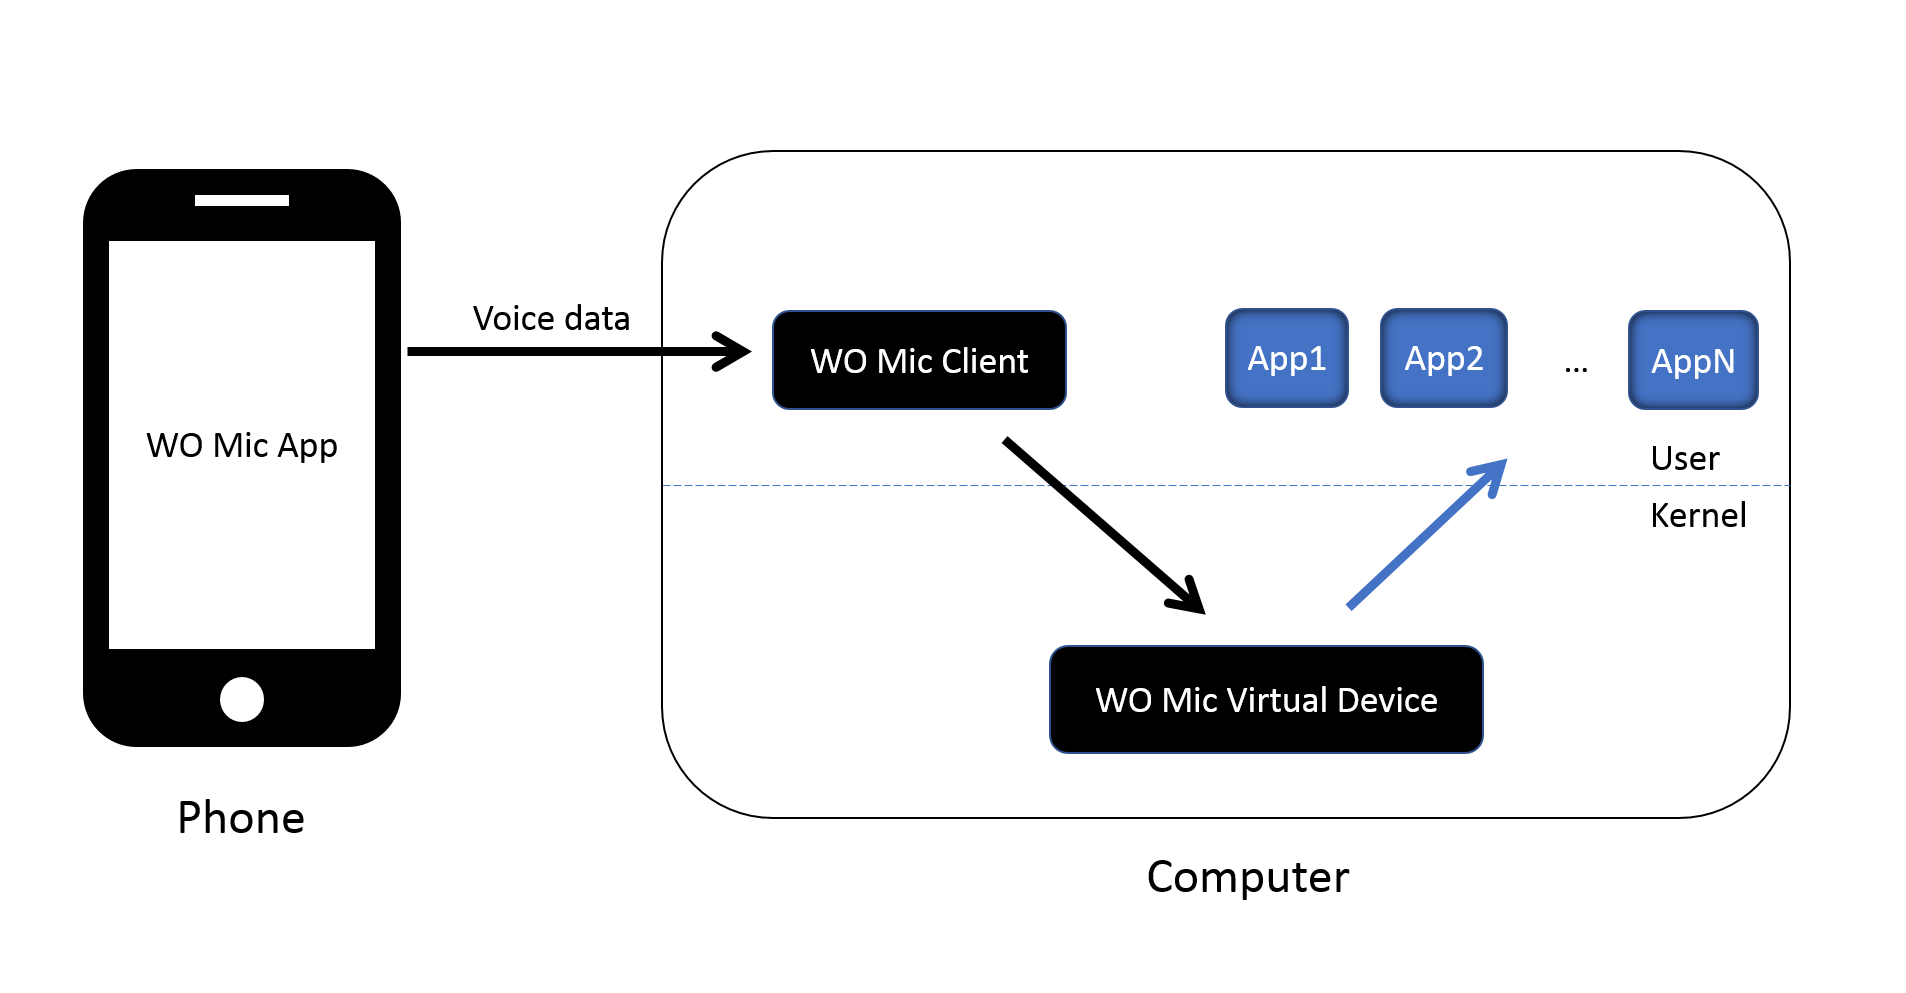
\includegraphics[width=0.65\textwidth]{Chapters/3CHP/Images/WOMICDiag.png}
    \caption{Flow of data in the components of the software\cite{WOMicFREE}}
    \label{fig:diagramWOMIC}
\end{figure}
In addition to this, is also necessary to install the drivers of the phone in use, if the connection is made over USB.\\
To save the acquired data, MatLab was used to record the data of the microphone from the desire time and saved in ".txt" files for further analysis. 
%%The following two paragraphs must go in other section
%%Insert flux gram here for a easy explanation and perception of the flow of information
A script in MatLab was developed in order to perform this measurements and the capture is made once at a time, but not all configurations are done over this script. To start, the phone is connected over USB to the computer, in the application at phone the transport selected must be \textbf{USB}, on the app settings and after that started the application, in the top right play shape button. 
%%Insert here instructions
In the computer the client software must be initialized and connected to the phone in the following order \textit{\>Connection\>Connect...} a new window will open, on which the \textbf{USB} must be selected as transport type and finalizing by pressing \textit{Connect}. In MATLAB the input correspondent to the microphone must be selected.\\
When this is done, the script runs and starts to record data from the microphone, for the desire amount of time. When the microphone starts to record, the surface of the LPG bottle is knocked and the captured signal is saved.
\section{??}
% \begin{figure}[!htb]
%     \centering 
%         \begin{subfigure}[c]{\textwidth}
%             \centering
%             \input{Sections/3Transforms/Images/DFTSymmetry.tex}
%             \caption{}
%             \label{subfig:dft}
%         \end{subfigure}
%         \begin{subfigure}[c]{0.45\textwidth}
%             \centering
%             \input{Sections/3Transforms/Images/DCT1Symmetry.tex}
%             \caption{}
%             \label{subfig:dct1}
%         \end{subfigure}
%         \begin{subfigure}[c]{0.45\textwidth}
%             \centering
%             \input{Sections/3Transforms/Images/DCT2Symmetry.tex}
%             \caption{}
%             \label{subfig:dct2}
%         \end{subfigure}
%         \begin{subfigure}[c]{0.45\textwidth}
%             \centering
%             \input{Sections/3Transforms/Images/DCT3Symmetry.tex}
%             \caption{}
%             \label{subfig:dct3}
%         \end{subfigure}
%         \begin{subfigure}[c]{0.45\textwidth}
%             \centering
%             \input{Sections/3Transforms/Images/DCT4Symmetry.tex}
%             \caption{}
%             \label{subfig:dct4}
%         \end{subfigure}
%         \caption{Sequences generated in the first step of Table \ref{tab:DFTDCT}for the DFT and different DCTs. Filled dots correspond to the original sequence ((a) - \emph{DFT}; (b)) - \emph{DCT-I}; (c)) - \emph{DCT-II}; (d)) - \emph{DCT-III}; (e)) - \emph{DCT-IV}).}
%     \label{fig:2NSeq}
% \end{figure}
% \begin{lstlisting}
%     ./aomenc <INPUT-FILE> -h <HEIGHT> -w <WIDTH> -o <OUTPUT-FILE> --limit=10 -p 1 --cpu-used=8 --i420 --q-hist=64 --end-usage=q --cq-level=<CQ-LEVEL>
% \end{lstlisting}
%\addcontentsline{toc}{section}{References}
